
\chapter{Constraints on Single-Cell Chemotactic Performance}

\noindent
In this chapter we examine the constraints that the external environment poses on single-cell chemotaxis. The work presented here is the product of a collaborative project with Dr.\ Bumsoo Han's group at Purdue University. In conjuction with Dr.\ Han and Hye-ran Moon's experiments on breast cancer cell chemotaxis, I developed a computational model of single-cell chemotaxis. From simulations we are able to predict how environmental parameters affect breast cancer cell chemotactic performance. Furthermore we use a simple physical model of chemotaxis to explain how environmental parameters vaired in experiments and simulations constraint chemotactic performance.

As mentioned in Chapter 1, chemotaxis can be broken down into cell sensing, polarization, and locomotion. How well the cell executes these aspects of chemotaxis determines its performance. Just as the fundamental limits to cell sensory precision is set by the extrinsic noise in chemical diffusion, chemotactic performance is limited by extrinsic and intrinsic parameters present in its three core components. The ability for the cell to polarize and induce motility is an intrinsic property of the particular cell-type in question, whereas environmental parameters affect what the cell can sense and its ability to move. Environmental parameters are independent of cell-type, and so provide extrinsic limits to chemotaxis. Here we focus solely on environmental parameters, and study how they place extrinsic limits on chemotactic performance. Although experiments are conducted on only one cell-type, we can focus on extrinsic constraints by fitting cell-dependent simulation and analytic parameters to observed experimental data.

Before presenting experimental, simulation, and theoretical results, the most prevalent chemotaxis metrics found in the literature are reviewed. This is important because a wide variety of metrics are used to measure the chemotactic performance. Different metrics may be used to characterize one aspect of chmeotaxis, and several metrics go by the same or very similar names. All metrics are dependent on the details of each experimental set-up to varying extents, and it is frequently unclear how different metrics can be compared or related between studies. This ambiguity makes identifying quantitative patterns between different studies very challenging. Effective chemotaxis crucially depends on adequate accuracy, persistence, and speed in cell dynamics. From the review three metrics are identified that provide a comprehensive and intuitive description of chemotactic behavior. With these metrics identified, we present the results from the breast cancer cell chemotaxis experiments performed by the Han group. Simulations of single-cell chemotaxis are used to probe beyond what is experimentally feasible, and identify the characteristic effects environmental parameters have on chemotactic performance. Finally, a simple analytical model is used to determine the extrinsic limits on cell chemotactic accuracy and persistence. Using experiment data we can fix the cell dependent parameters of the analytical model and predict a constrained phase-space in chemotactic accuracy and precision.

\begin{figure}
    \centering
    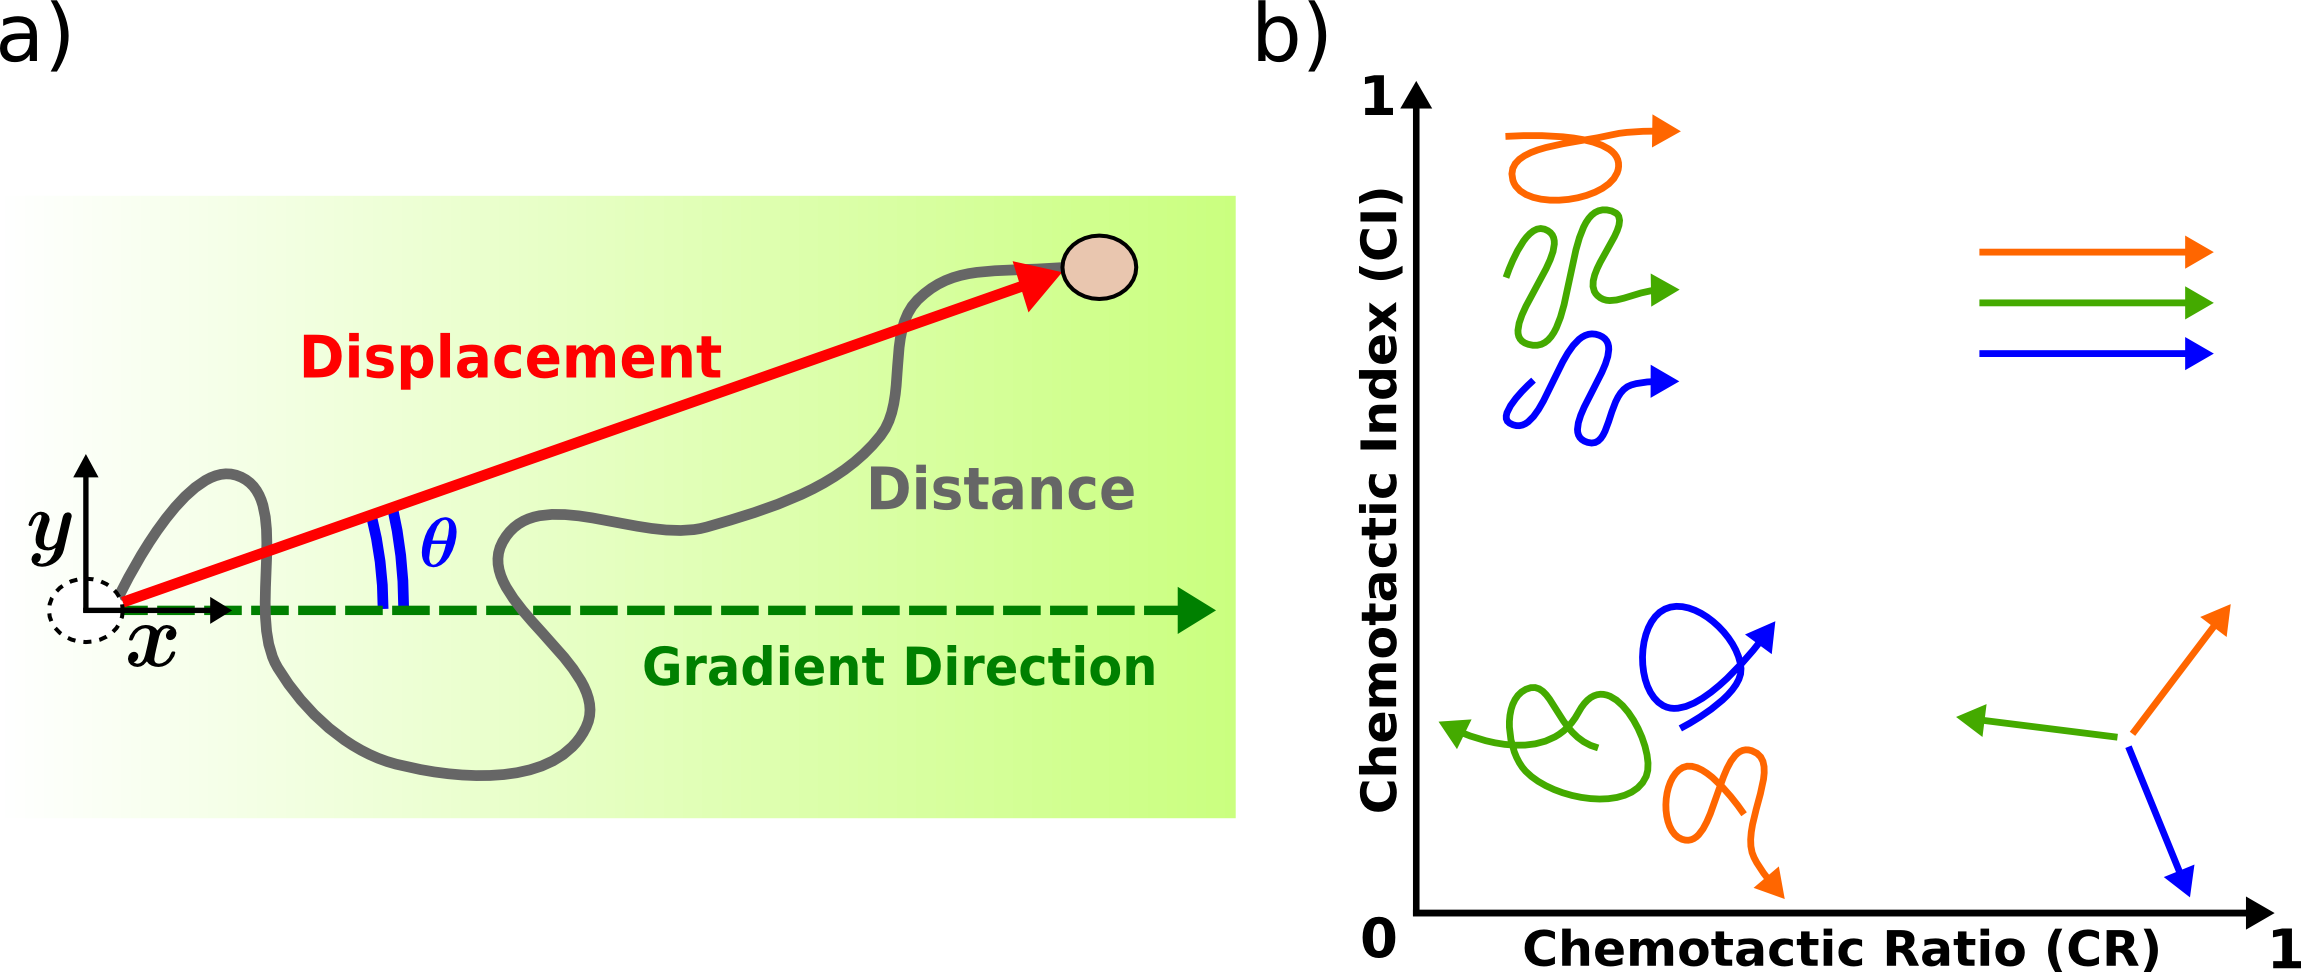
\includegraphics[width=0.90\textwidth]{../fig/ch2_fig1.png}
    \caption{a) Illustration of cell chemotaxis. The cell's displacement makes an angle $\theta$ with the gradient direction. b) Illustration of cell trajectories associated with different CI and CR values. Illustrations of typical cell trajectories are shown in different colors.} \label{fig:ch2_1}
\end{figure}


\section{Review of Chemotaxis Metrics}

The literature on cell migration and chemotaxis experiments contains a variety of different metrics used to characterize cell motion. In this section we briefly review some of the more common metrics used for measuring cell motility, persistence (also referred to as directionality) and chemotactic performance. Common metrics from the literature and their definitions are explained in order to motivate the metrics used in our study.

\subsection{Accuracy}

For chemotaxis experiments, often a single metric typically referred to as the chemotactic index is reported to quantify how well cells track the chemoattractant in question. However, the mathematical definition of the chemotactic index (CI) varies throughout the literature, the most common definitions are listed. CI has been defined as the ratio of the distance traveled towards the chemoattractant to the distance traveled in the absence of chemoattractant \cite{nelson1975chemotaxis}, the ratio of the number of cells that migrate in response to a chemical to the number of cells that migrate in the absence of stimulus \cite{iellem2001unique,mayr2002vascular,fiedler2005vegf}, and the population average of the cosine of the angle made between a cell's displacement and the gradient direction
\cite{funamoto2001role,mouneimne2006spatial,van2007biased,kay2008changing}.

The former two ratio-based definitions are commonly found in the literature although comparing them between different experiments is difficult. Both definitions give a measure of the migratory response when cells are exposed to a certain chemical. They may confound the effects of chemokinesis and chemotaxis since the former induces cell motility but not necessarily directed migration. Exposure to a motility inducing chemical will increase the response the cells have and thereby increasing CI, although cellular response may not be directed. Furthermore, neither definition clearly characterizes the cell's accuracy in tracking the chemoattractant; instead they quantify a fraction of cells that respond to the chemical and this does not capture any information about the cells' directedness. In the case of these two metrics $\text{CI} = 1$ corresponds to no chemotactic response and $\text{CI} > 1$ represents an increased response. Since CI here is unbounded, getting physical intuition for various values that are greater than one is difficult.

In this study we use the definition based on cosine of the angle cell trajectories make with the chemoattractant gradient direction as illustrated in Fig.\ \ref{fig:ch2_1}a. Specifically, we define CI as the population average of the cosine of the angle made between a cell's displacement and the gradient direction \cite{mouneimne2006spatial,kay2008changing,funamoto2001role},
\begin{equation} \label{eq:defCI}
    \text{CI} \equiv \langle \cos \theta \rangle \ .
\end{equation}
Strictly speaking, CI is bounded between -1 and 1, but for chemotaxis in response to a chemoattractant -- as is the case in this study -- CI generally falls between 0 and 1. $\text{CI} = 1$ represents perfectly accurate chemotaxis in which cell displacement is parallel to the gradient direction (Fig.\ \ref{fig:ch2_1}b, top-half), and $\text{CI} = 0$ indicates that the cells' migration is unbiased (Fig.\ \ref{fig:ch2_1}b, bottom-half). Having a bounded metrics makes it easy to compare different values of CI and get an intuitive picture for the type of cell dynamics it represents. The bounded nature of Eq.\ \ref{eq:defCI} along with its clear characterization of accuracy make it superior to the ratio-based definitions of CI, and this metric is also more easily comparable between experiments.

\subsection{Persistence}

Cell migratory persistence is commonly quantified using the chemotactic ratio and the directional autocorrelation function. The chemotactic ratio (CR) is defined as the ratio of the cell's displacement to the total distance traveled (Fig.\ \ref{fig:ch2_1}a):
\begin{equation} \label{eq:defCR}
    \text{CR} \equiv  \left\langle \frac{\text{displacement}}{\text{distance}} \right\rangle \ .
\end{equation}
The CR metric goes by several names in the literature such as the McCutcheon index \cite{mccutcheon1946chemotaxis}, directionality (ratio), length ratio \cite{gorelik2014quantitative}, and straightness index \cite{codling2008random}.
CR is bounded between 0 and 1 and intuitive sense can be made of either limit. If $\text{CR} = 1$, then the cells are moving in perfectly straight lines and motion is optimally efficient (Fig.\ \ref{fig:ch2_1}b, right-half). However, $\text{CR} = 0$ represents cell motion that is neither persistent nor efficient (Fig.\ \ref{fig:ch2_1}b, left-half).

The directional autocorrelation function (AC) calculates on average, how much time must pass for the cell's current direction of motion to be independent from the direction it was going in the past \cite{gorelik2014quantitative,dang2013inhibitory}.
It quantifies persistence by calculating the timescale of decay in correlations between current and previous direction of motion.
The AC is defined as
\begin{equation} \label{eq:AC1}
    \text{AC}(\Delta t) = \langle \cos(\theta_{\Delta t + t}-\theta_{t}) \rangle_{t,N} \ ,
\end{equation}
with $\Delta t$ the time difference between two points in a trajectory and the average in Eq.\ \ref{eq:AC1} is taken over all starting times $t$ and all $N$ cell trajectories. The AC measures how the direction of cell motion along one trajectory is correlated with the direction of motion at a time $\Delta t$ later.
At $\Delta t = 0$, $\text{AC}(0) = 1$ since when no time has passed both angles in Eq.\ \ref{eq:AC1} are in fact the same. In the opposite limit, when a very large amoint of time has passed
$\text{AC}(\Delta t \to \infty) = 0$,
since trajectories that occurred infinitely far apart in time have no effect on each other. Calculating AC for all $\Delta t$ times sets a timescale $\tau$ which quantifies the rate at which correlations decay from 1 to 0. Therefore $\tau$ quantifies the persistence in the cells motion, a larger $\tau$ is indicative of more persistent motion. We define $\tau$ as
\begin{equation} \label{eq:tau1}
    \tau = \int_0^\infty dt' \ \text{AC}(t') \ .
\end{equation}
The AC is useful for cross-comparing experiments since the persistence timescale $\tau$ is largely independent of the frequency at which measurements were taken as well as the total observation time. However, the timescale $\tau$ obtained from the AC is not a bounded dimensionless quantity unlike CR. For this reason we choose to use CR as the persistence metric over AC, and we discuss the validity of this choice after presenting the experimental results in Sect.\ 2.2.

% \begin{figure}[ht]
%     \centering
%     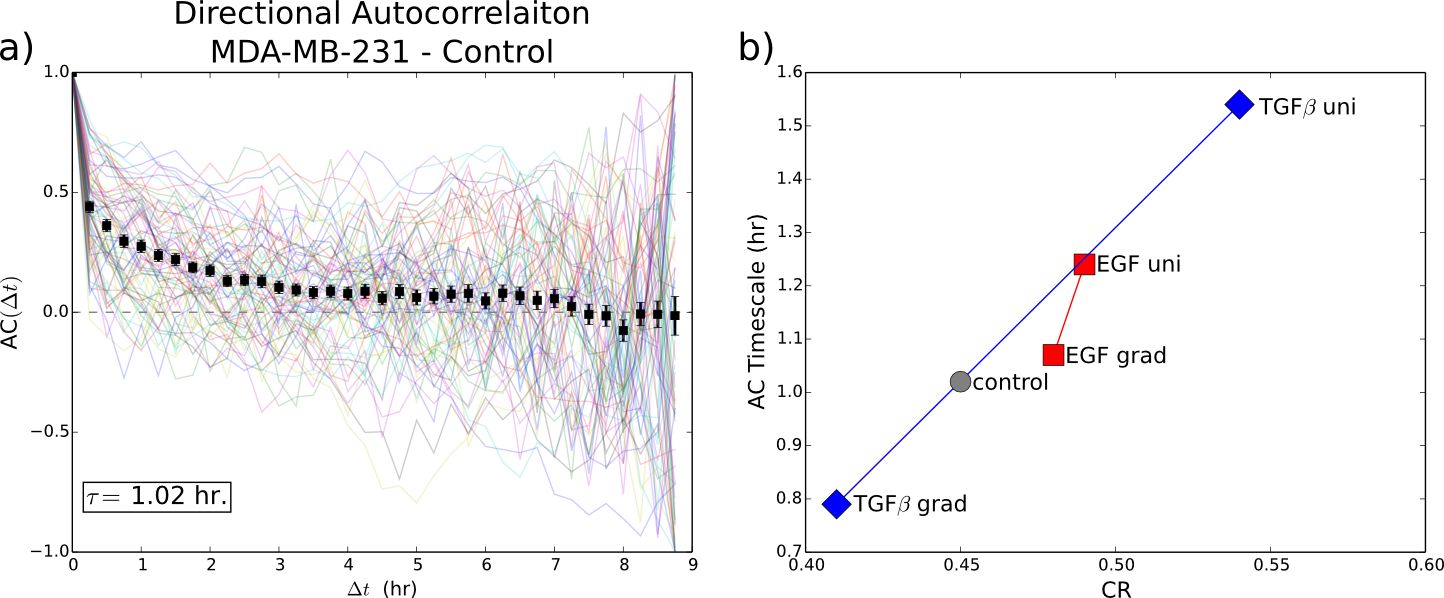
\includegraphics[width=0.80\textwidth]{../fig/ch2_fig5.png}
%     \caption{a) Directional Autocorrelation from control dataset. Light-colored trajectories indicate autocorrelations for individual cell trajectories. Timescale $\tau$ is calculated using Eq.\ \ref{eq:tau1}. b) Directional autocorrelation timescales and CR values for all experimental assays. Data points are color-coded based on chemical environment.} \label{fig:ch2_5}
% \end{figure}
%
% We calculate the AC and its timescale $\tau$ from our experimental data. Fig.\ \ref{fig:ch2_5}a shows the autocorrelations from the control assay, the black dots are the AC values for all times $\Delta t$ observed in our experiment, and its AC has a timescale
% $\tau = 1.02 \ \text{hr}$.
% In Fig.\ \ref{fig:ch2_5}b we compare the CR and AC timescale values from all experimental conditions. Going from a uniform to a graded concentration of either EGF or TGF$\beta$ results in a decreased CR value, and the AC timescale also decreases when going from a uniform to a graded concentration. This indicates that there is a monotonic relationship between CR and $\tau$. As the measured value of CR increases so too will the AC timescale $\tau$.
%
% Therefore, quantifying persistence with CR leads to the same patterns and analysis that could have been deduced from using AC. Additionally, the timescale obtained from the AC is not a bounded, dimensionless quantity. This makes gaining intuition about persistence from the autocorrelation timescale more difficult than CR. Since CR provides a clearer intuitive picture for persistence in cell chemotaxis we use it in our study.

\subsection{Migration Speed}

The final factor contributing to chemotactic performance is cell speed. Speed is important in order to ensure that the cells reach their destination in a timely manner. Cell speed is affected by many environmental factors such as collgen stiffness, and chemical concentration profiles. We define speed as the population average of the instantaneous cell speed during chemotaxis
\begin{equation}
    \bar{v} \equiv \left\langle \frac{||\Delta\vec{r}||}{\Delta t} \right\rangle \ ,
\end{equation}
with $\Delta t$ being the time lapsed between observations, and $||\Delta\vec{r}||$ the cell's displacement during that time period.
Experimentally, measuring cell speed is limited by the frequency at which cell trajectories are recorded. Therefore comparison of cell speed recorded in different chemotaxis studies necessitates careful consideration of the procedures used in each respective study. Nonetheless, speed is a simple, easily digestible metric for quantifying how motile cells are during chemotaxis.


\section{Experimental Results}

\begin{figure}
    \centering
    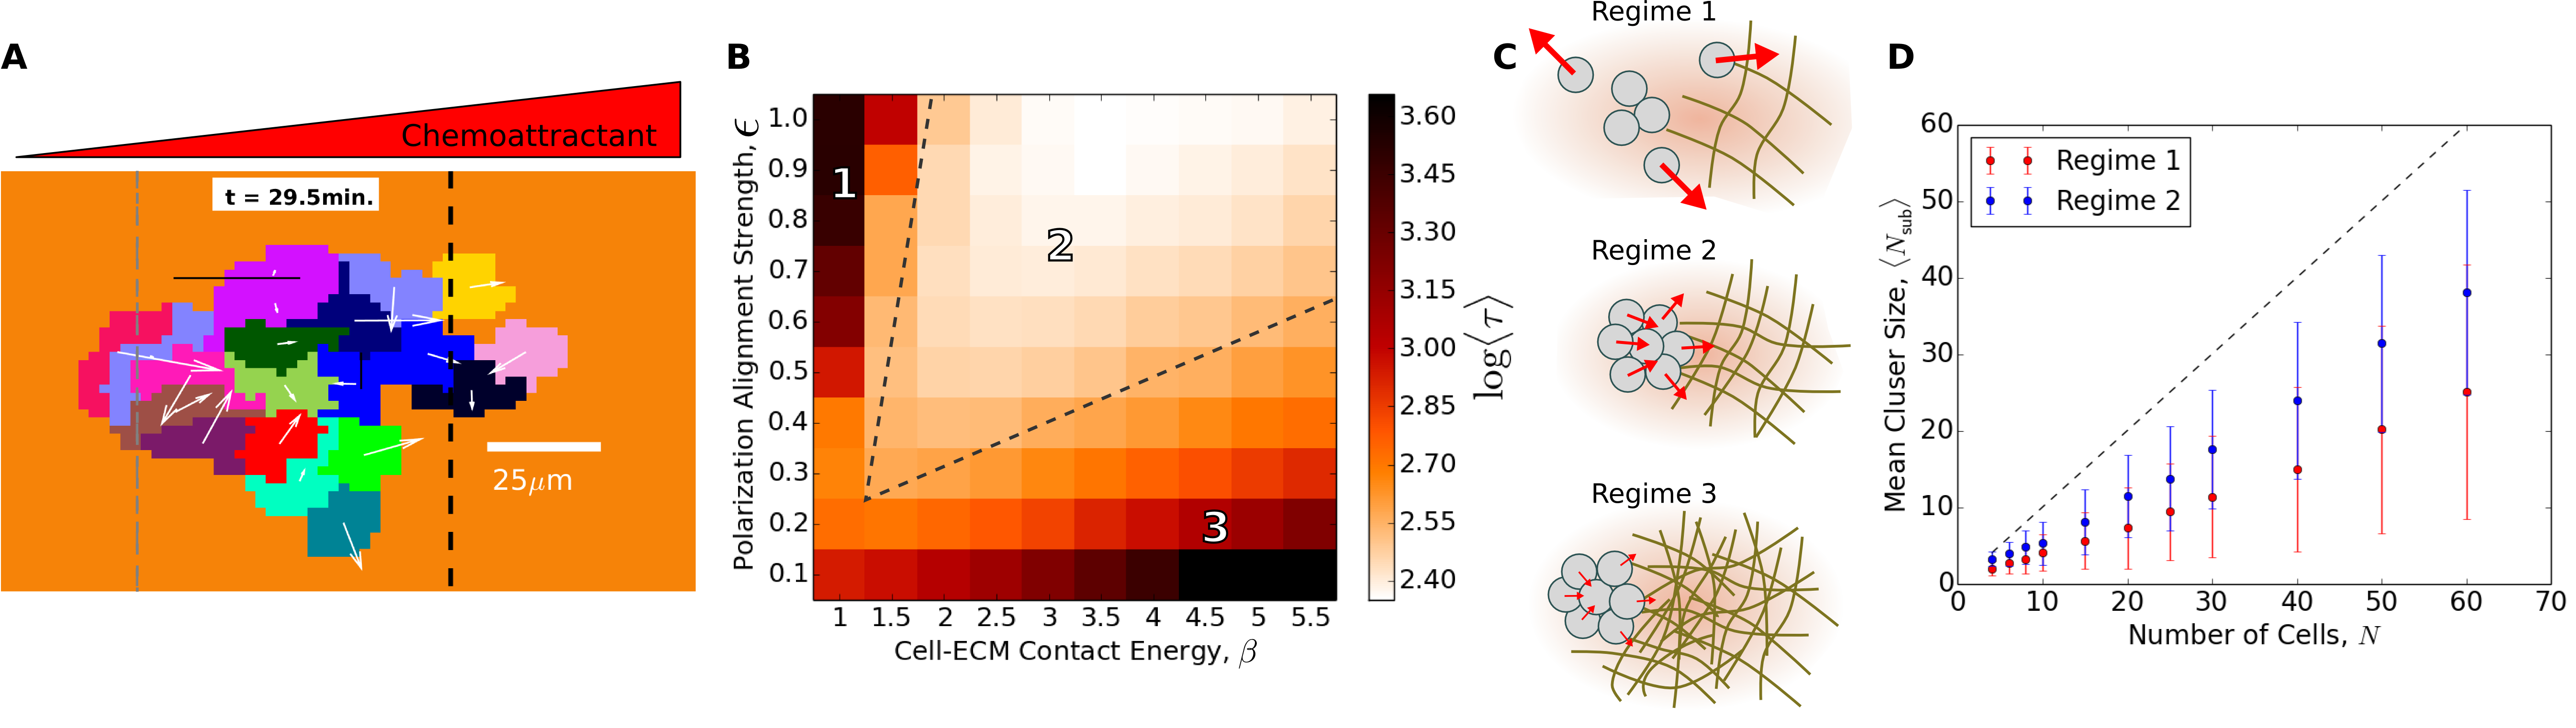
\includegraphics[width=0.90\textwidth]{../fig/ch2_fig2.png}
    \caption{Human breast cancer MDA-MB-231 cell chemotaxis assays. Cells are cultured in different chemical environments and trajectories are tracked. CI (a), CR (b) and mean speed ($\bar{v}$) are reported. d) Summary of chemotaxis assay results, data point size is proportional to mean speed. In all plots colors: no chemoattractant (gray), 400nM EGF uniform concentration (red), 0-800nM EGF gradient (orange), 25nM TGF$\beta$ uniform concentration (blue), and 0-50nM TGF$\beta$ gradient (light blue). Error bars are the standard error over the population of trajectories observed.} \label{fig:ch2_2}
\end{figure}

The Han group conducted experiments to measure the effects that the environment imposes on cell chemotaxis. Different chemicals known to induce motility and directed migration were used to measure how chemotactic performance would change. Human breast cancer cell line MDA-MB-231 was used in several different chemotaxis and motility assays.

Experiments are conducted in a soft lithography fabricated microfluidic device. The device contains three channels, two side channels and a center channel. Side channels are connected to reservoirs in order to control the chemical profile present in the center channel. The center channel consists of collagen in which MDA-MB-231 cells are placed. The cells are cultured in the collagen for 48 hours followed by a 24 hour serum starvation period. Afterwards, concentrations of the chemoattractant of interest are added to the side channels. The concentration differences between the side channels creats a gradient through the collagen in the center channel. With the chemoattractant added to the device, images of the cells are taken every 15 minutes for a total 8 hour duration in order to obtain single-cell chemotaxis trajectories. \r{Add a figure of experimental device / set-up.}

First, a control experiment was conducted to characterize the baseline behavior of the MDA-MB-231 cells (Fig.\ \ref{fig:ch2_2}, gray bars). As expected, when the cells are not in the presence of a chemoattractant they do not migrate in any preferred direction as indicated by a chemotactic index centered around zero (Fig.\ \ref{fig:ch2_2}a). However, even in the absence of any chemical signal cells do exhibit persistent motion with a $\text{CR} > 0$ (Fig.\ \ref{fig:ch2_2}b), since the cell motion is intrinsically directional due to the cells' internal migratory machinery \cite{petrie2009random}.
Similar persistent motion has been observed and modeled in the context of other cell types \cite{kim2013cooperative,codling2008random,othmer1988models}. Finally, we characterize the baseline cell motility, with a speed of $\approx 12 \mu\text{m/hr}$ (Fig.\ \ref{fig:ch2_2}c).

What happens when chemicals are added to the external environment? We start by performing assays with epidermal growth factor (EGF). EGF is a known motility inducing agent \cite{kim2013cooperative,mosadegh2008epidermal} and may also bias cell migration \cite{wang2004differential}. Experiments are conducted for both a uniform 400nM concentration and gradient of 0-800nM across a 1mm-long chamber.
As shown in Fig.\ \ref{fig:ch2_2}a, adding a uniform concentration of EGF to the cellular environment results in a CI value within one standard error of $\text{CI} = 0$ indicative that the addition of EGF does not produce any significant bias to cell trajectories. This is expected since adding a uniform concentration of a chemical should not bias cell motion.
On the other hand, adding a gradient of EGF does produce a CI that is signficantly above zero meaning the breast cancer cells do chemotax in response to EGF (Fig.\ \ref{fig:ch2_2}a).
Examining the persistence and speed of cell movement (Fig.\ \ref{fig:ch2_2}b-c) shows that the uniform concentration gives similar results to the graded concentration. We observe that adding EGF results in about a 6\% increase in CR and an increased cell speed in agreement with the literature that EGF induces cell motility.

Next we used transforming growth factor type beta (TGF$\beta$) as a chemoattractant. TGF$\beta$ is a known chemoattractant for many cell types \cite{wahl1987transforming,bischoff1997chemotaxis}.
It is also involved in development, inflammation, and may be involved in carcinogenesis \cite{clark1998molecules,javelaud2004mammalian,pang2016tgf}.
Here we find that TGF$\beta$ is a strong chemoattractant (Fig.\ \ref{fig:ch2_2}a, light-blue) with $\text{CI} = 0.278 \pm 0.075$ when a 0-50nM gradient is used. TGF$\beta$ does promote more directionally persistent motion as its CR value for a uniform concentration (but not for the graded concentration) is greater than that recorded for the control (Fig.\ \ref{fig:ch2_2}b). Adding TGF$\beta$ to the cellular environment does improve cell speed, but not to the extent that was observed for motility-inducing EGF (Fig.\ \ref{fig:ch2_2}c).

\begin{figure}[ht]
    \centering
    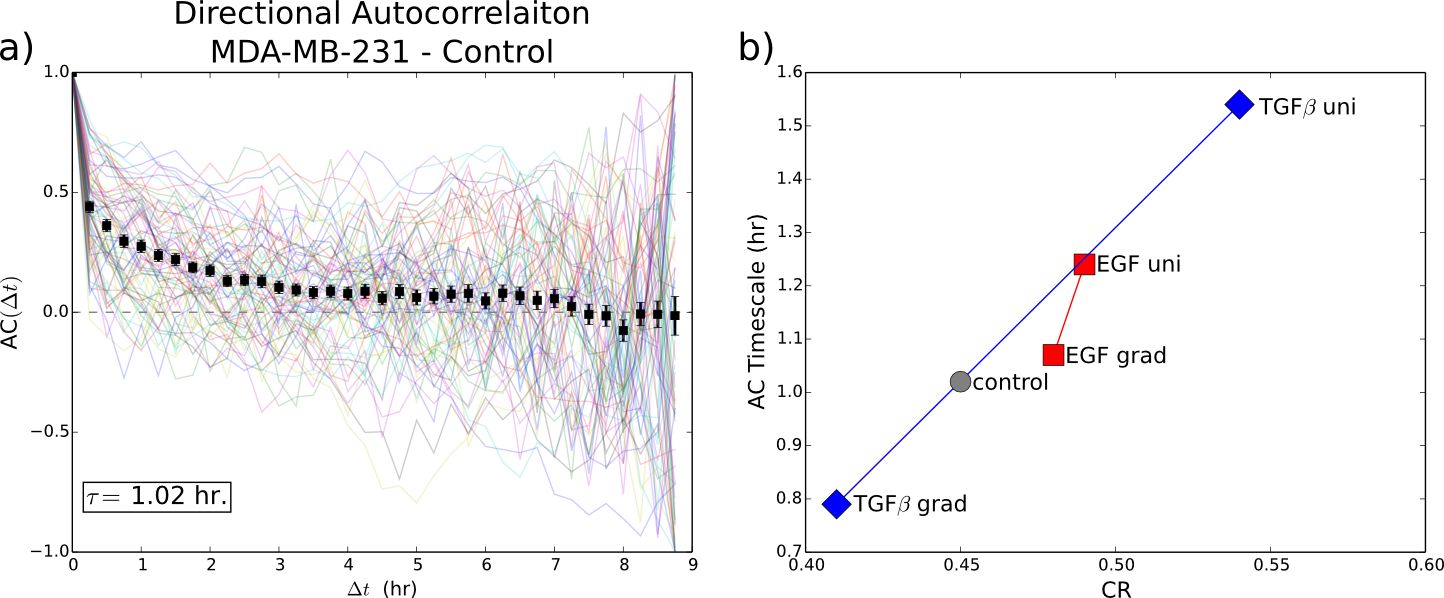
\includegraphics[width=0.80\textwidth]{../fig/ch2_fig5.png}
    \caption{a) Directional Autocorrelation from control dataset. Light-colored trajectories indicate autocorrelations for individual cell trajectories. Timescale $\tau$ is calculated using Eq.\ \ref{eq:tau1}. b) Directional autocorrelation timescales and CR values for all experimental assays. Data points are color-coded based on chemical environment.} \label{fig:ch2_5}
\end{figure}

For all experimental conditions we calculate the AC and its timescale $\tau$ in order to verify the validity in using the CR as the persitence metric instead of the AC timescale. Fig.\ \ref{fig:ch2_5}a shows the autocorrelations from the control assay, the black dots are the AC values for all times $\Delta t$ observed in our experiment, and its AC has a timescale
$\tau = 1.02 \ \text{hr}$.
In Fig.\ \ref{fig:ch2_5}b we compare the CR and AC timescale values from all experimental conditions. Going from a uniform to a graded concentration of either EGF or TGF$\beta$ results in a decreased CR value, and the AC timescale also decreases when going from a uniform to a graded concentration. This indicates that there is a monotonic relationship between CR and $\tau$. As the measured value of CR increases so too will the AC timescale $\tau$.
Therefore, quantifying persistence with CR leads to the same patterns, analysis, and conclusions that could have been deduced from using AC. Since CR provides a bounded dimensionless metric with clear intuition we use it in our analysis.

In summary, adding a gradient of EGF or TGF$\beta$ results in chemotaxis as indicated by CI values significantly above zero. The experimental parameters' affects on chemotactic behavior are consolidated into Fig.\ \ref{fig:ch2_2}d. Movement in the CI-CR plane of Fig.\ \ref{fig:ch2_2}d indicates changing persitence and accuracy of chemotaxis, whereas the size of each data point represents the average speed. Under all conditions the cells move at speeds of $\sim 10 \mu\text{m}/\text{hr}$. An increase in speed is observed when the MD-MB-231 cells are exposed to either growth factor. This is not not a surprising result since chemical agents that promote persistent or directed migration often results in increased motility \cite{petrie2009random}. EGF and TGF$\beta$ both produce similarly persistent motion though EGF promotes more motility as indicated by its fastest cell speed.


\section{Chemotaxis Simulations}

The experiments tell us how cells respond to specific concentration profiles of EGF and TGF$\beta$. However, experiments do not tell us how chemotactic performance varies from experimental configuration to the next, and we are limited to testing conditions that experimentally feasible. Can we develop a model of chemotaxis that is capable of predicting chemotactic performance before doing experiments?

Here we conduct single cell chemotaxis simulations to further probe cell chemotactic performance. With simulations environmental parameters such as collagen stiffness, background chemical concentration, and gradient can all be easily varied over a wide range of values which may not be experimentally practical. These experimental parameters are individually varied to develop predictions on how each each parameter affects chemotactic accuracy (CI), persistence (CR), and speed.


\subsection{Computational Implementation}

\begin{figure}
    \centering
    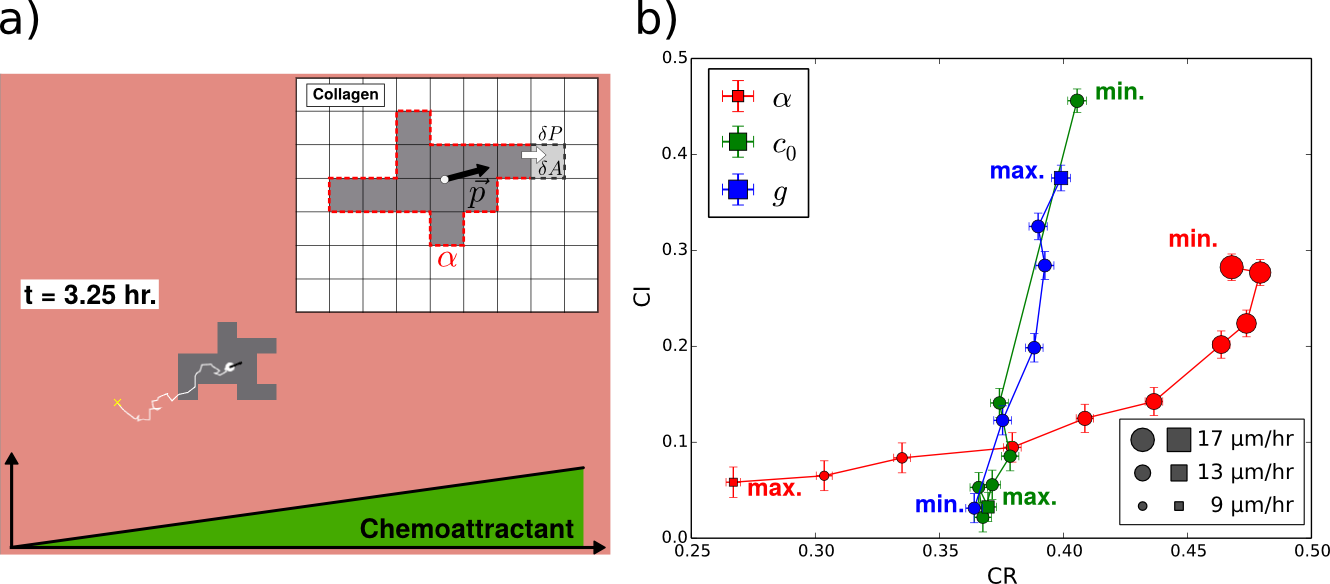
\includegraphics[width=0.80\textwidth]{../fig/ch2_fig3.png}
    \caption{a) Screen shot of simulation. Cell (gray) is migrating towards increasing chemical concentration, and the white line traces out the cell's path. Inset, illustration of the CPM. A Cell is comprised of simply connected lattice sites. There is an adhesion energy associated with cell-collagen contact, $\alpha$ (red-dashed line). Cell motility occurs through the addtion/removal of lattice sites (light-gray). The white dot represents the cell's center of mass and the black arrow its polarization vector $\vec{p}$. b) Simulation results. Environmental parameters collagen stiffness $\alpha$ (red), background concentration $c_0$ (green), and gradient $g$ are varied (blue).
    Parameter values along each trajectory: $\alpha \in \{ 0.1, 0.4, 0.7, 1.0 \}, c_0 \in \{ 1.0, 10.0, 100.0 \ \text{nM} \}, g \in \{ 1.0, 5.0, 10.0 \ \text{nM}/\mu\text{m} \}$.}
    \label{fig:ch2_3}
\end{figure}

Cell chemotaxis simulations are implemented using the Cellular Potts Model (CPM) \cite{graner1992simulation,swat2012multi}. The CPM is a lattice based simulation implementation. Cells are comprised of lattice sites, and cells move and fluctuate in shape by the stochastic addition or removal of lattice sites.
Cells are defined as a finite set of simply connected lattice sites $\{ x \}$ (Fig.\ \ref{fig:ch2_3}a, inset).
Cell lattice sites are given the lattice label $\sigma(x)=1$ whereas the extracellular environment is labeled $\sigma(x)=0$. Cells have a desired size $A_0$ and perimeter $P_0$ from which they can fluctuate, and cells adhere to their neighboring environment with an adhesion energy $\alpha$. The energy of the whole system is the sum of adhesion, area-restriction, and perimeter-restriction terms,
\begin{equation} \label{eq:CPMu1}
    u = \alpha P + \lambda_A(A_0 - N)^2 + \lambda_P(P_0 - P)^2 \ .
\end{equation}
$A$ is the cell area, and $P$ is the cell's perimeter. The parameters $\lambda_{A}$ and $\lambda_{P}$ are the area and perimeter restriction costs.

Cell motion is a consequence of minimizing the energy of the whole system. This stochastic process is sensitive to thermal fluctuations and is modeled using a Monte Carlo scheme. In a system of $n$ lattice sites, one \textit{Monte Carlo} time step (MC step) is composed of $n$ attempts to copy a random lattice site's label to a randomly chosen neighboring site. An attempt is accepted with probability $\mathcal{P}$, which depends on the change in the system's energy $\Delta u$ accrued in copying over the lattice label,
\begin{equation} \label{eq:ch2_prob}
    \mathcal{P} =
    \begin{cases}
        e^{-\left( \Delta u - w \right)} &\ \Delta u - w > 0 , \\
        1 &\ \Delta u - w \leq 0 .
    \end{cases}
\end{equation}
The bias term $w$ acts to bias cell motion in the direction of its polarization, and is necessary in order for cells to exhibit directed motion \cite{szabo2010collective}.
The bias is defined as
\begin{equation}
    w = \Delta\hat{x} \cdot \vec{p} \ ,
\end{equation}
with $\Delta\hat{x}$ the unit vector pointing in the change in the cell's center of mass caused by the addition or removal of the lattice site in question, and $\vec{p}$ is the cell's polarization vector (Fig.\ \ref{fig:ch2_3}a, black arrow). The dot product acts to bias cell motion since movement that is parallel to the polarization vector will result in a more positive $w$ which in turn results in a higher acceptance probability (Eq.\ \ref{eq:ch2_prob}).

After the random addition and removal of lattice sites occurs during one MC step the cell updates its polarization vector. The time evolution of the cell's polarization vector is defined as
\begin{equation} \label{eq:CPMp1}
    \frac{d\vec{p}}{dt} = -r\vec{p} + \Delta\vec{x} + \epsilon \vec{q}\ .
\end{equation}
The first term in Eq.\ \ref{eq:CPMp1} results in exponential decay of the cell's current polarization at a rate $r$. $\Delta x$ is the cell's displacement and it creates persistence in cell motion; $\vec{p}$ is reinforced in the direction of motion. The third term represents chemotaxis, with $\epsilon$ the bias strength and $\vec{q}$ an abstraction of the cell's gradient sensing.
\begin{equation} \label{eq:CPMq1}
    \vec{q} = \frac{1}{N_P} \sum_{i=1}^{N_P} \frac{c_i-\bar{c}}{\bar{c}} \ \hat{r}_i
\end{equation}
The sum is taken over all $N_P$ lattice sites which comprise the perimeter of the cell. $\hat{r}_i$ is a unit vector that points radially outwards from the cell's center of mass to the location of lattice site $i$. $c_i$ is the concentration of the chemoattractant sampled at the lattice site $i$ and $\bar{c}$ is the cell's measurement of the mean concentration in its local environment; $c_i$ is sampled from a Poisson distribution and $\bar{c}$ is the mean from all $c_i$ measured at each lattice site.

The CPM used here is similar to that used in our previously published study on collective cell chemotaxis \cite{varennes2016collective}. The source code for the single-cell chemotaxis simulations can be found here \cite{ch2code}.

\subsection{Calibration of Simulation Parameters}

The length and time scales of the simulation are calibrated to the experimentally observed average cell size and speed over all assays. Internal cellular parameters, such as the cell polarization strength and decay rate, are then calibrated such that the simulation's CI and CR values are approximately the same as those observed in experiments.

From experiments we know that cells are on average $400 \mu\text{m}^2$ in size, and we use this to set one lattice site to equal $5 \mu\text{m}$ such that cells occupy $\sim 10$ lattice sites. Next we calibrate the time-scale in simulations by equating the average cell velocity in simulations to approximately that observed experimentally, $\sim 10 \mu\text{m/hr}$. With this we equate a simulation time step to $5 \text{min}$. Finally, we need to calibrate the internal cell parameters. We consider internal cell parameters to be those which are not affected by the environment and are characteristic of the particular cell type we are simulating.
These include the energy costs of cell area and perimeter fluctuations $\lambda_A$, $\lambda_P$, the polarization decay rate $r$, and the bias strength $\epsilon$. These parameters are set such that the chemotactic index (CI) and chemotactic ratio (CR) recorded in experiments is approximately the same as that observed in experiments. We refer to the collagen stiffness $\alpha$, background concentration $c_0$, and the concentration gradient $g$ as experimental parameters.

In running simulations internal parameters are fixed to the values used for the initial calibration. External parameters are varied in order to quantify their effects on chemotactic performance. The internal parameter values used as well as the baseline external parameter values are listed in Table \ref{table:ch2_1}.


\begin{table}[ht]
\begin{center}
\begin{tabular}{ |c|c|c| }
\hline
Parameter & Value & Notes \\ \hline
Relaxed Cell Area $A_0$ & $400 \ \mu\text{m}^2$ & \\ \hline
Relaxed Cell Perimeter $P_0$ & $3.6\sqrt{A_0} \ \mu\text{m}$ & Assumes circular resting shape \\ \hline
Area Energy Cost $\lambda_A$ & 0.3  & Prevents ``stringy'' cell-shapes \\
Perimeter Energy Cost $\lambda_P$ & 0.01 & \\ \hline
Polarization Bias Strength $\epsilon$ & 0.1 & \\ \hline
Polarization Decay Rate $r$ & $2.4 \ \text{hr}^{-1}$ & Sets polarization memory time \\ \hline \hline
Cell-environment Contact Energy $\alpha$ & 0.7 & Sets energy scale \\ \hline
Concentration $\bar{c}$ & $10 \ \text{nM}$ & \\
Gradient $g$ & $0.5 \ \text{nM/}\mu\text{m}$ & \\ \hline
\end{tabular}
\caption{Table of parameters and values used in simulations. The first six parameters are intrinsic to the cell and remain fixed. The final three parameters represent the environment and are varied in Fig.\ \ref{fig:ch2_3}. Energy costs are in units of $k_B T$, where $k_B T$ is the thermal energy of the CPM Monte Carlo scheme.}
\label{table:ch2_1}
\end{center}
\end{table}


\subsection{Simulation Results}

With length and time scales of the simulation are calibrated and internal cellular parameters fixed, we vary the environmental parameters. Collagen stiffness $\alpha$, background concentration $c_0$, and gradient $g$ are varied to study their effects on chemotactic performance. Fig.\ \ref{fig:ch2_3}b shows the resulting CI, CR and speed values when environmental parameters are changed. Each data point along a parameter's trajectory indicates the CI and CR values, while the size of the data point indicates the average speed for that particular choice of parameter value. All other parameters are held fixed along each trajectory. The background concentration is varied over three orders of magnitude whereas both the gradient and collagen stiffness are varied over one order of magnitude.

We find that varying the background concentration and gradient most significantly affects the accuracy of chemotaxis, not the persistence nor the speed. This is displayed in Fig.\ \ref{fig:ch2_3}b in which both $c_0$ and $g$ have much longer trajectories along the CI axis than along either the speed or CR axis.
As the background concentration increases, the fluctuations in the diffusing chemoattractant become larger relative to the gradient making it more difficult for the cell to correctly determine the gradient direction. This results in a decreasing CI as $c_0$ increases. Conversely, increasing the gradient enables the cell to more accurately detect the gradient direction resulting in increasing CI values (Fig.\ \ref{fig:ch2_3}b,c).

Along with changing the accuracy of chemotaxis, varying $c_0$ and $g$ also results in slightly increased persistence and speed. This goes hand in hand with the improved gradient detection due to increased $g$ or decreased $c_0$. As cells become more accurate movements perpendicular to the gradient are reduced, resulting in more persistent and faster motion along the gradient direction as shown in Fig.\ \ref{fig:ch2_3}b.

Collagen stiffness is the only parameter that significantly affects the persistence in the cell's motion, indicated by the larger displacement in $\alpha$'s trajectory along CR versus CI or speed (Fig.\ \ref{fig:ch2_3}a,b). Stiffer collagen is more difficult for cells to traverse leading to slower speeds, and we find a monotonic relationship between CR and speed when stiffness is varied (Fig.\ \ref{fig:ch2_3}b). As was observed for the chemoattractant-related parameters the more persistent cell motion seen at small $\alpha$ also corresponds to more accurate, faster chemotaxis.

From these simulation results we deduce some stereotypical patterns of cell chemotaxis. Increasing the relative change in chemoattractant concentration across cell (either by increasing $g$ or reducing $c_0$) results in more accurate chemotaxis. Material that is more difficult for cells to traverse during chemotaxis, whether its stiffer colagen \textit{in vitro} or denser extracellular matrix \textit{in vivo}, results in reduced chemotactic performance across all metrics. Finally, the simulations show a positive correlation between CR and speed since as cell motion becomes more persistent it typically also enables faster cell movement.

\section{Analytical Model of Chemotaxis}

Interestingly, although both experiments and simulations vary environmental parameters affecting cell chemotaxis, the chemotactic performance metrics do not dramatically change. Both CI and CR can range from 0 to 1, but our MDA-MB 231 cell assays result in CR values close to 0.45 and CI values less than 0.3 for all environmental conditions (Fig.\ \ref{fig:ch2_2}). Simulations allow for probing chemotactic behavior over an even larger parameter space, and yet CI and CR values remain limited to a fraction of the whole range (Fig.\ \ref{fig:ch2_3}).

Can this phenomenon be explained with a simple physical model? One of the simplest models for cell movement and chemotaxis is the biased persistent random walk \cite{alt1980biased,othmer1988models}. In its simplest form, a random walk involves a walker that is equally likely to move in any direction, and its next movement is independent of its previous motion. To add persistence to the random walk means that the walkers' movements are correlated. The walker's next movement is not equally likely in all directions as in the simplest case, but now depends on its previous direction of motion \cite{patlak1953random}. Finally, adding bias means that the walker is more likely to move in a particular fixed direction.
Biased persistent random walks (BPRWs) have been used to model chemotaxis \cite{alt1980biased,othmer1988models}. Before we get into how the BPRW model can shed light on the chemotactic performance of MDA-MB-231 breast cancer cells, lets review the model formulation.

\subsection{Biased Persistent Random Walk Formulation}

The BPRW is modeled as a velocity jump process in which a walker moves in a particular direction with fixed speed for an exponentially distributed amount of time. The walker reorients to a new direction $\vec{v}$ from its previous velocity $\vec{v}'$ depending on the probability density $T(\vec{v},\vec{v}')$. We assume a reorientation frequency $\lambda$, thus $\lambda^{-1}$ is the average run time, and that it moves at a constant speed $s$. The reorientations are chosen based on a probability density $T(\vec{v},\vec{v}')$ which depends only on the angular direction of the walker's movements $T(\vec{v},\vec{v}') = T(\theta,\theta')$. Here $\theta$ is taken relative to the $x$ axis which is parallel to the gradient direction.

Let $p(\vec{r},\theta,t) d\vec{r} d\theta$ be the number density of individual walkers found between positions $\vec{r}$ and $\vec{r}+d\vec{r}$ with movement orientation between $\theta$ and $\theta + d\theta$. From Othmer \textit{et al}.\ \cite{othmer1988models} it is shown that the evolution equation for the probability density $p(\vec{r},\theta,t)$ simplifies to
\begin{equation} \label{eq:p1}
    \frac{\partial p}{\partial t} + s \vec{\xi}\cdot\vec{\nabla} p =
    -\lambda p + \lambda \int_{-\pi}^{\pi} d\theta' \ T(\theta,\theta') \ p(\vec{r},\theta,t) \ ,
\end{equation}
with $\vec{\xi} = (\cos\theta,\sin\theta)$. In order to derive expressions for the moments some assumptions have to made on the reorientation probability density. We assume that $T(\theta,\theta')$ is the sum of two functions,
\begin{equation} \label{eq:t1}
    T(\theta,\theta') = \underbrace{k(\theta)}_\text{bias}
    + \underbrace{h(\phi)}_\text{persistence}
\end{equation}
with $\phi = \theta - \theta'$ being the turning angle. $k(\theta)$ is maximally valued and symmetric about $\theta = 0$, and biases movement towards the gradient. $h(\phi)$ is the turning angle distribution which is assumed to be symmetric about $\phi = 0$. Along with these properties $T(\theta,\theta')$ and its component functions must obey the following conditions:
\begin{align} \label{eq:t2}
    &T(\theta,\theta') \geq 0 \ , \text{for all } (\theta,\theta') \ , \\
    \int_{-\pi}^{\pi} d\theta \ &T(\theta,\theta') = 1 \ , \label{eq:t3} \\
    \int_{-\pi}^{\pi} d\theta  \ &k(\theta)         = 0 \ , \label{eq:t4} \\
    \int_{-\pi}^{\pi} d\phi    \ &h(\phi)           = 1 \ . \label{eq:t5}
\end{align}

With Eq.\ \ref{eq:p1} and the restrictions on $T(\theta,\theta')$ (Eq.\ \ref{eq:t2}-\ref{eq:t5}), Othmer \textit{et al}.\ \cite{othmer1988models} derive the moments for the BPRW.
\begin{align} \label{eq:moment1}
    \begin{split}
    \langle r^2(t) \rangle &= \frac{2s^2}{\lambda_0} \left[ \left(1-\frac{2\chi^2}{(1-\psi)^2}\right)t
    - \frac{\chi^2 t e^{-\lambda_0 t}}{(1-\psi)^2}
    + \frac{3\chi^2(1-\psi)^{-2}-1}{\lambda_0} \left(1-e^{-\lambda_0 t}\right)
    \right. \\
    &\qquad \left.
    + \frac{\chi^2 \lambda_0 t^2}{2(1-\psi)^2} \right]
    \end{split} \\
    \langle x(t) \rangle &= \frac{\chi}{1-\psi} s \left(t -\frac{1-e^{-\lambda_0 t}}{\lambda_0} \right) \label{eq:moment2} \\
    \langle y(t) \rangle &= 0 \label{eq:moment3}
\end{align}
These results are derived with the assumption that individuals in the BPRW start at the origin with uniformly distributed initial orientations.
The mean squared displacement (Eq.\ \ref{eq:moment1}) and the mean walker location (Eq.\ \ref{eq:moment2}-\ref{eq:moment3}) both depend on the parameters $\chi$, $\psi$, and $\lambda_0$. The bias strength (also referred to as the taxis coefficient) is represented by $\chi$ which is defined as
\begin{equation} \label{eq:chi}
    \chi \equiv \int_{-\pi}^{\pi} d\theta \ k(\theta) \ \cos\theta \ .
\end{equation}
$\psi$ represents the persistence strength (also referred to as the persistence index), and it is defined as
\begin{equation} \label{eq:psi}
    \psi \equiv \int_{-\pi}^{\pi} d\phi \ h(\phi) \ \cos\phi \ .
\end{equation}
Note that the restrictions on the reorientation probability density (Eq.\ \ref{eq:t2}-\ref{eq:t5}) result in $\chi \leq 1 - \psi$. Fianlly, $\lambda_0$ is the effective turning rate of the walker,
$\lambda_0 \equiv \lambda(1-\psi)$.
Since $\lambda$ is the reorientation rate and $\psi$ is the persistence strength, $\lambda_0$ describes the effective rate at which the walker forgets its previous orientation.

Starting from the definitions for CI and CR in Eqs.\ \ref{eq:defCI}-\ref{eq:defCR}, we use the moments given in Eqs.\ \ref{eq:moment1}-\ref{eq:moment3} to calculate CI and CR for the BPRW model as functions of time:
\begin{align} \label{eq:ci1}
    \text{CI}(t) &= \left\langle \frac{x}{r} \right\rangle \approx
    \frac{\langle x \rangle}{\sqrt{\langle r^2 \rangle}}
    = \chi \sqrt{\frac{\lambda}{2(1-\psi)}} \left(t -\frac{1-e^{-\lambda_0 t}}{\lambda_0} \right) \
    [ \ \ldots \ ]^{-1/2} \ , \\
    \text{CR}(t) &= \frac{\langle r \rangle}{L} \approx
    \frac{\sqrt{\langle r^2 \rangle}}{st}
    = \frac{1}{t}\sqrt{\frac{2}{\lambda_0}} \
    [ \ \ldots \ ]^{1/2} \ .
    \label{eq:cr1}
\end{align}
The term $[ \ \ldots \ ]$ is shorthand for the bracketed term in Eq.\ \ref{eq:moment1}, and $L$ is the total path length. In Eq.\ \ref{eq:ci1} we approximate the two moments as being independent of one another, and in both Eqs.\ \ref{eq:ci1}-\ref{eq:cr1} we make the approximation that
$\langle x \rangle \approx \sqrt{\langle x^2 \rangle}$.
These approximations are in very good agreement the exact solutions of CI and CR times in which many reorientation events occur, $t \gg \lambda^{-1}$. Note that neither CI nor CR depend on the speed $s$, and assuming that $\chi < 1 - \psi$, to first order CR decays as $\text{CR} \sim t^{-1/2}$.

The BPRW predictions for CI and CR depend on how strongly persistence and bias affect the walker's movements. The timescales in the BRPW are calibrated to those of our experiments; total observation time $t = 9 \text{hr}$, the reorientation frequency
$\lambda = 4 \text{hr}^{-1}$), and we approximate the speed to be
$s = 15 \mu\text{m/hr}$. With the BPRW timescales calibrated we can proceed to vary $T(\theta,\theta')$ which in turn affects the bias strength $\chi$, and the persistence strength $\psi$.

\begin{figure}[ht]
    \centering
    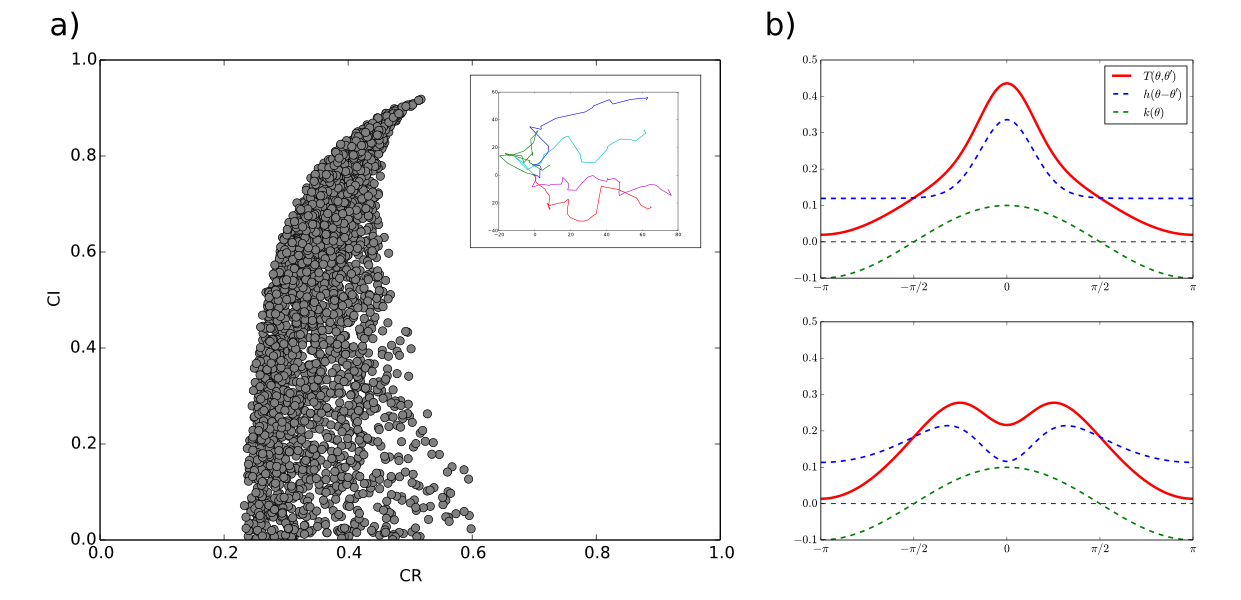
\includegraphics[width=0.80\textwidth]{../fig/ch2_fig6.png}
    \caption{a) Possible values of CI and CR for a BPRW. Each dot represents the CI and CR value for a BPRW of a given bias and persistence strength. Inset, sample trajectories of a BPRW. b) Example reorientation probability densities $T(\theta,\theta')$, and their component bias $k(\theta$) and persistence $h(\theta-\theta')$ functions. For both b) plots $\theta'=0$. For all plots: $t =36$, $\lambda = 1.0$, $s = 3.75$, and $\theta=0$ is the direction of bias.}
    \label{fig:ch2_6}
\end{figure}

Simulations of the BPRW are performed with varying $T(\theta,\theta')$ to find the resulting values of CI and CR possible given our experimental system. In the simulations the bias and persistence functions to take on the forms:
\begin{align}
    k(\theta) &= k_1 \cos\theta \ , \\
    h(\theta-\theta') &= h_1 f_\text{VM}(\theta | \ \theta', \kappa_1) + h_2 f_\text{VM}(\theta | \ \theta', \kappa_2) \ .
\end{align}
Here $k_1$ sets the bias strength, and $h(\theta-\theta')$ is a linear combination of two von Mises distributions with
$f_\text{VM}(\theta | \ \theta', \kappa) = \frac{1}{2\pi I_0(\kappa)} e^{\kappa \cos(\theta-\theta')}$.
The von Mises distribution is approximately equal to a normal distribution bounded to a circle, and it is commonly used in random walk models of biological systems \cite{codling2008random}.
The parameters $\kappa_1$ and $\kappa_2$ set the persistence strength with larger values of $\kappa$ resulting in higher persistence. $h_1$ and $h_2$ set the shape of the distribution, with $\{h_1,h_2\} > 0$ results in a single-peaked $h(\theta-\theta')$ function as shown in Fig.\ \ref{fig:ch2_6}b, top. Whereas, if $h_1> 0$ and $h_2<0$ then the resulting $h(\theta-\theta')$ function has two peaks, symmetric across $\theta=\theta'$ (Fig.\ \ref{fig:ch2_6}b, bottom).
Interestingly, even in this idealized model of chemotaxis the whole range of CI and CR values is not available to the BPRW. The mechanics of the random walk limit its performance resulting in behavior that cannot attain perfect accuracy ($\text{CI}=1$), nor perfect persistence ($\text{CR}=1$).

In summary, by calibrating BPRW to our experiments the parameters $t$, $\lambda$, and $s$ are fixed. From here we can sample possible CI and CR values given a particular bias and persistence strength. By varying over all possible combinations of bias and persistence parameters while enforcing the restrictions on $T(\theta,\theta')$ (Eq.\ \ref{eq:t2}-\ref{eq:t3}) all possible values of CI and CR permitted under the BPRW model are calculated. The CI and CR values permitted by our theoretical model are shown alongside the experimental results in  Fig.\ \ref{fig:ch2_4}. We see that our simple theoretical model is able to recover the CI and CR values observed. More importantly, the BPRW puts limits on how well these breast cancer cells can chemotaxis regardless of how favorable the environmental conditions are made as represented by the gray-shaded region in Fig.\ \ref{fig:ch2_4}.

\begin{figure}
    \centering
    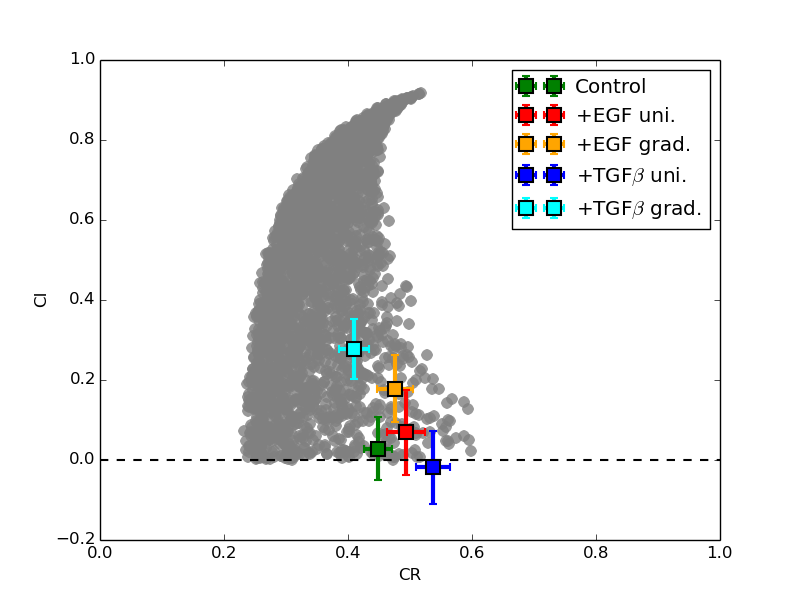
\includegraphics[width=0.80\textwidth]{../fig/ch2_fig4.png}
    \caption{Theoretical bounds on chemotactic performance based on the biased persistent random walk model. Gray dots represent possible theoretical CI and CR values for a BPRW. Colored squares are experimentally recorded values for different environmental conditions.} \label{fig:ch2_4}
\end{figure}
